\subsection{Photoelectron Trajectories}

	The electrons emitted from the spacecraft due to the photoelectric effect, have a kinetic
	energy corresponding to a Maxwellian distribution with a temperature of \(T_{ph} =  3.8481\cdot 10^{4} \text{K}\).
	Figure~\ref{fig:trajectories} illustrates the trajectories of the emitted electrons in simulation \(6\).
	As the probes are situated \(10 \text{cm}\) to the sides of the spacecraft on the \(x-\)axis, the probes
	may be hit by the photo-emitted electrons. In the following section, \ref{sec:acc_emitted}, we show the number of electrons hitting
	the probes.


	\begin{figure}
		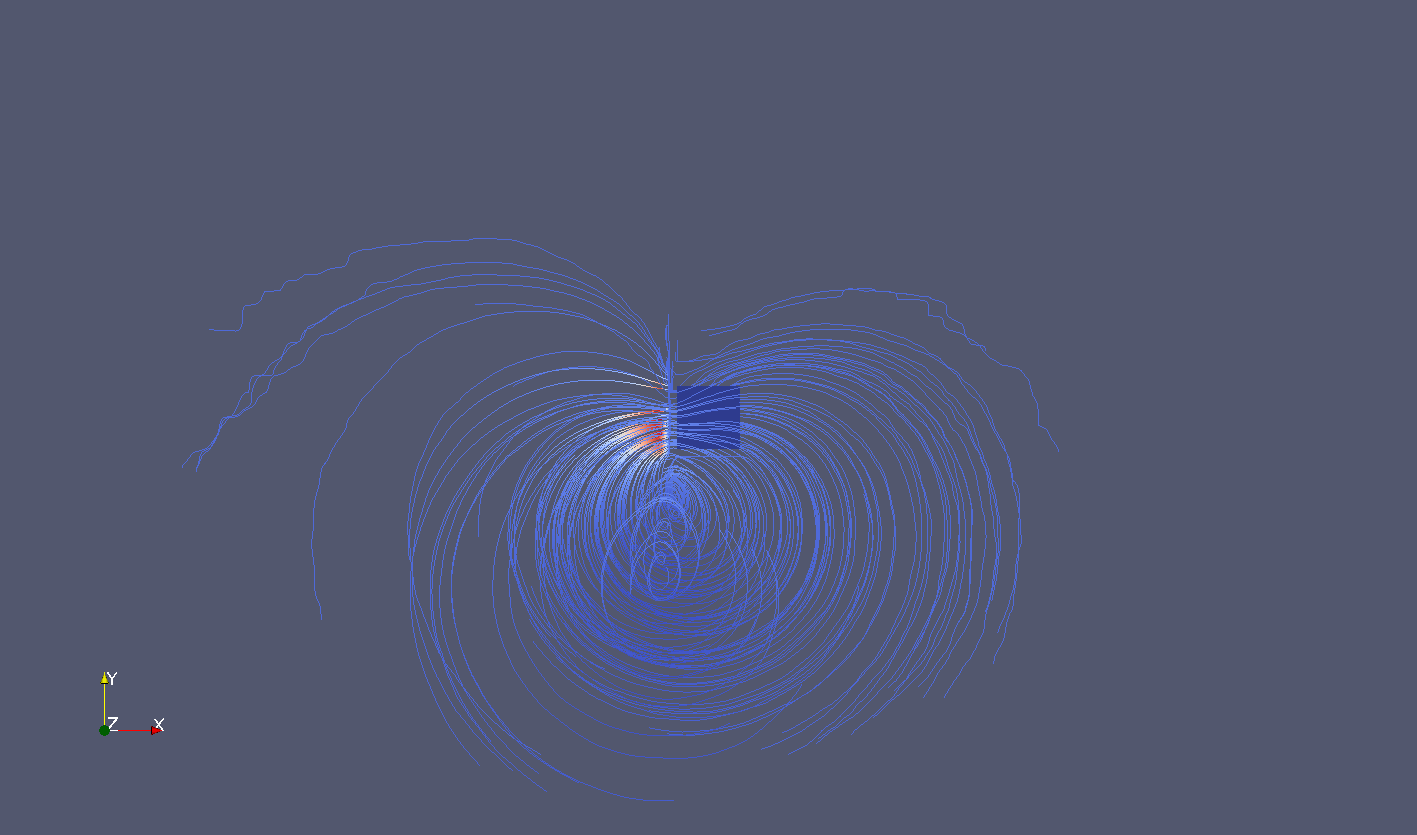
\includegraphics[width = 0.49 \textwidth]{images/case6_jph_paths}
		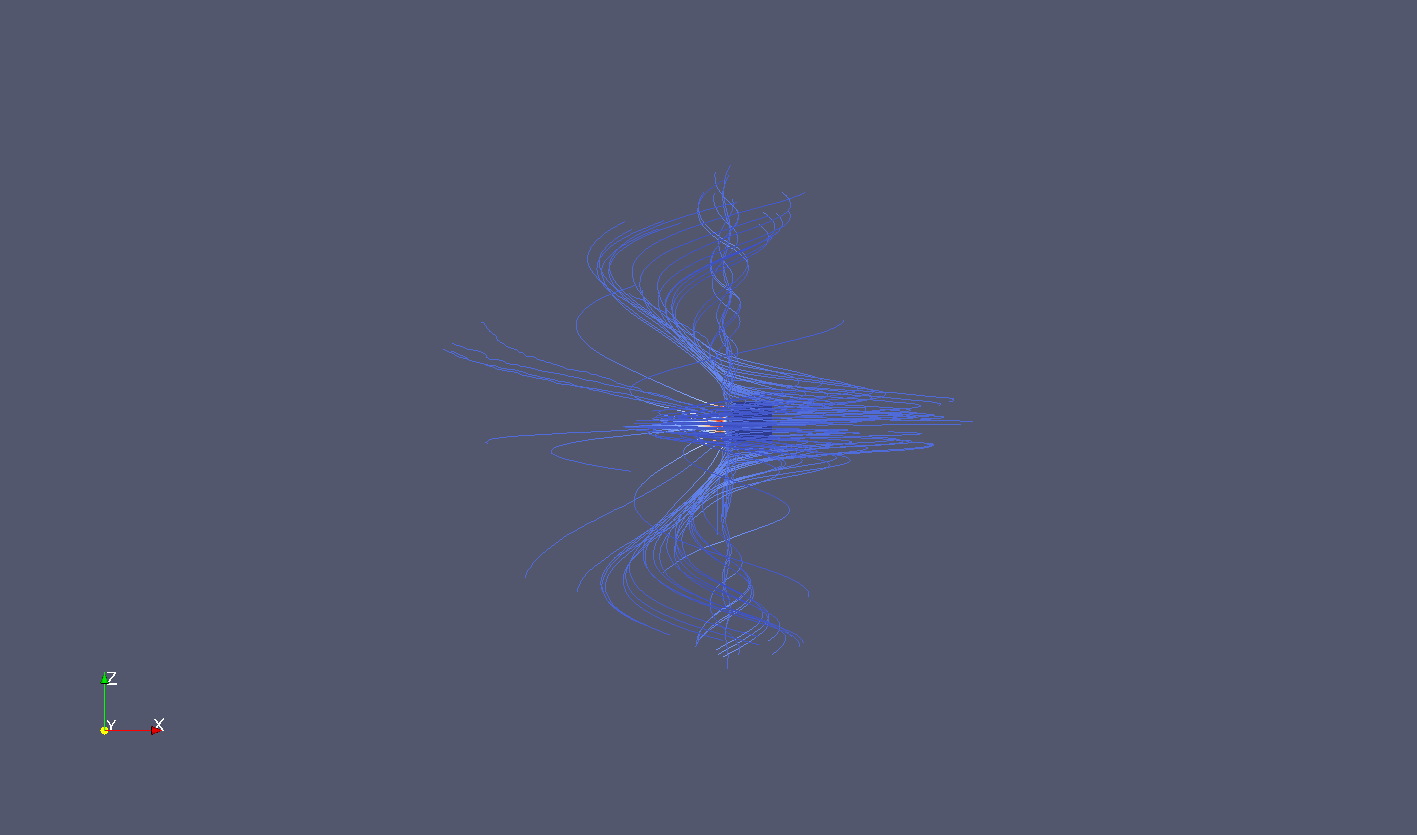
\includegraphics[width = 0.49 \textwidth]{images/case6_jph_paths_2}
		\caption{The trajectories of the electrons emitted by the photoelectric effect in simulation \(6\). The possible
		paths of the photoemitted electrons coincide with the volume occupied by the langmuir probes. The photoemitted electrons are strongly affected by the magnetic
		field \(\vec{B}\), and follows a gyrating path guided by \(\vec{B}\). The photoemitted electrons are in all the studied cases
		emitted from the spacecraft in \(-x\) direction, and the paths are similar. The langmuir probes are situated \(10 \text{cm}\) to each side
		of the spacecraft along the \(x-\)direction.}
		\label{fig:trajectories}
	\end{figure}

\subsection{Accumulated Photoelectrons on Langmuir Probes}
\label{sec:acc_emitted}

In the simulations both electrons and photoelectrons are absorbed by the probes. Table~\ref{tab:elec_current} shows the current
of both regular electrons, as well as photoelectrons, interacting with the probes.
The photoelectrons are emitted on the left side of the spacecraft and we see a larger current of
photoelectrons here. The current caused by the photoemission is \(10-100\) smaller than the current
from the electrons in the plasma. This photoelectrons may

\begin{figure}[h]
	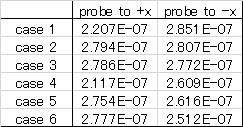
\includegraphics[width = 0.45\textwidth]{images/caliculation_of_electron_current}
	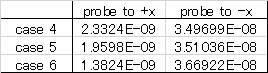
\includegraphics[width = 0.45\textwidth]{images/caliculation_of_PE_current}
	\caption{The left table shows the electron current (A) hitting the inserted probes at
	for the simulated cases \(1-6\). On the table to the right the photoelectrons hitting the probes are shown.
	The photoelectron current is smaller than the electron current from the plasma, varying from \(10-100\) times smaller.}
	\label{tab:elec_current}
\end{figure}


\subsection{Spacecraft Potential}
\begin{table}
\begin{center}
    \begin{tabular}{ | l | l | l | p{5cm} |}
    \hline
     & Without flow & With flow  \\ \hline
     Without Photon emission & -0.893   & -0.792 \\ \hline
     With Photon emission & -0.718 & -0.662 \\
    \hline
    \end{tabular}
	\caption{The potential, in \(V\), of the spacecraft computed with the thin sheet approximation, \ref{sec:theo_calc}.}
\end{center}
\end{table}

There is a difference between the theoretical and numerical potential, see section \ref{sec:pot_diff} for the numerical results, because $\lambda_D$ is not much
smaller then the length of the satellite, which is an assumption in the thin sheet approximation.
From these calculations we can, however, expect the potential over the spacecraft to rise
in the cases where we have photon emission.

\subsection{Induced electric current}
	%Redo this part if necessary
	The plasma is flowing in in relation to the coordinate system in the simulations.
	Due to this an induced electrical field, \(\varepsilon\), will appear.
	The induced electrical field, \(\varepsilon\), will balance the magnetic part of the Lorentz force,  \(\vec{v}\times \vec{B}\).
	Combined with the electrostatic approximation we can obtain the \(\varepsilon\).

	\begin{equation}
		\vec{\varepsilon} = \vec{v_D}\times \vec{B}
	\end{equation}

	This will cause a potential gradient perpendicular to the plasma flow and the magnetic field,
	using the electrostatic approximation we obtain the magnitude of the gradient.

	\begin{equation}
		\int{Edx} = -\phi
	\end{equation}

	\begin{equation}
		\phi = -\int \vec{v}_d\times\vec{B} \approx -\int \left( 41600 \text{m/s}\cdot 50E-6 \text{T} \right) dx
	\end{equation}
	\begin{equation}
		|\nabla\phi| = 2.08 \text{m}^{-1}
	\end{equation}

	\begin{figure}
		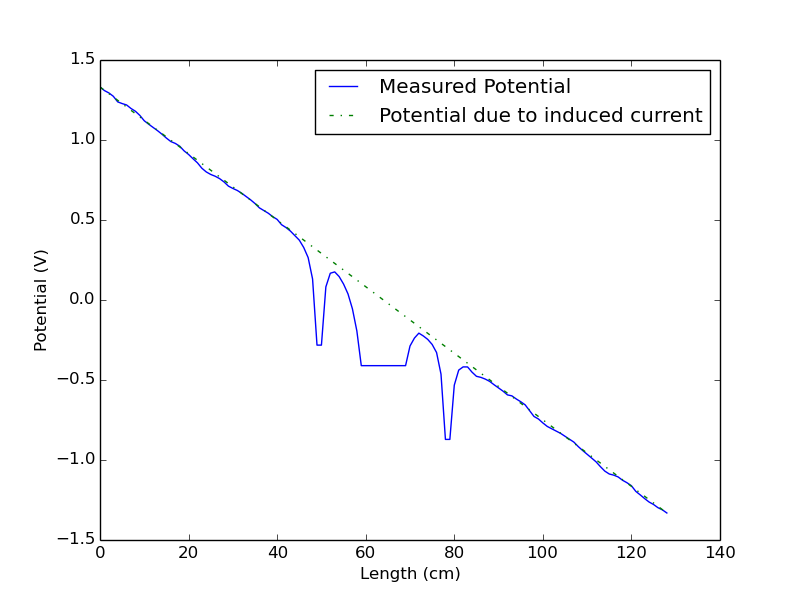
\includegraphics[width = \textwidth]{images/emph}
		\caption{The blue line is the potential along direction x for simulation \(6\). In this case the potential gradient is along
		the \(x-\)axis. The dotted green line is the potential caused by the induced electrical field. This should be accounted for
		if  we want to find the potential at the spacecraft and the probes.}
		\label{fig:emph}
	\end{figure}

	Figure~\ref{fig:emph} shows the measured potential at case \(6\). In section \ref{sec:pot_diff},  we compare
	the cases where the flow is in the same direction to avoid having to correct for this effect.

\subsection{Ion Density}
		The spacecraft is moving relative to the plasma flow, this causes a wake to be formed in the vicinity of the craft.
	 	Figures~\ref{fig:wake} illustrates the flow in case \(1,2\) and \(3\). In case \(1\) the right probe is in the wake,
		and in both the other cases the two probes aren't affected by the wake.

	    \begin{figure}
	        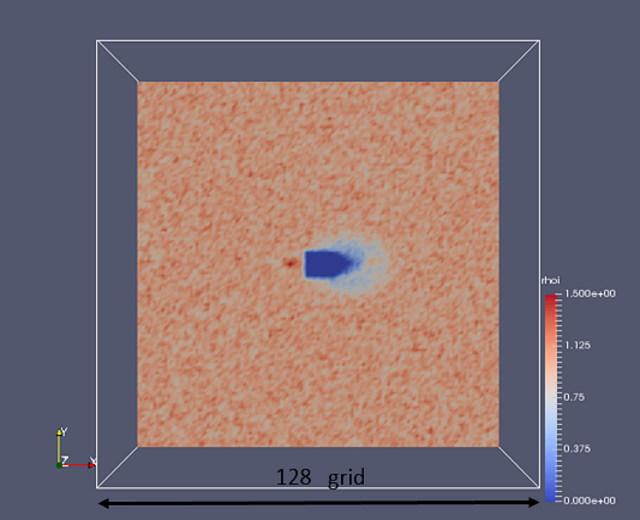
\includegraphics[width = 0.5\textwidth]{images/case1}
	        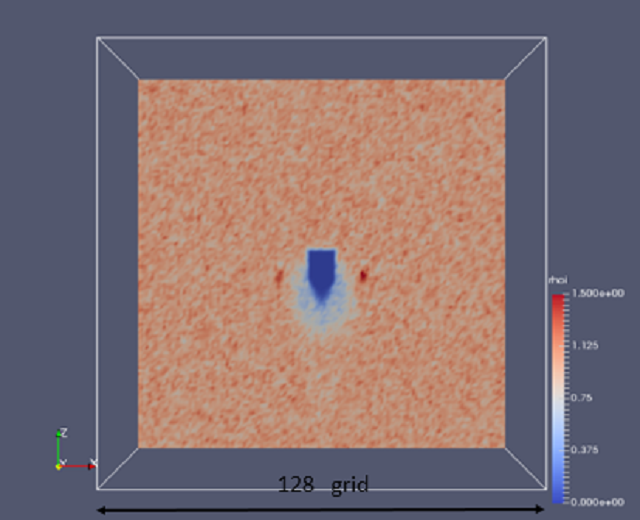
\includegraphics[width = 0.5\textwidth]{images/case2}
			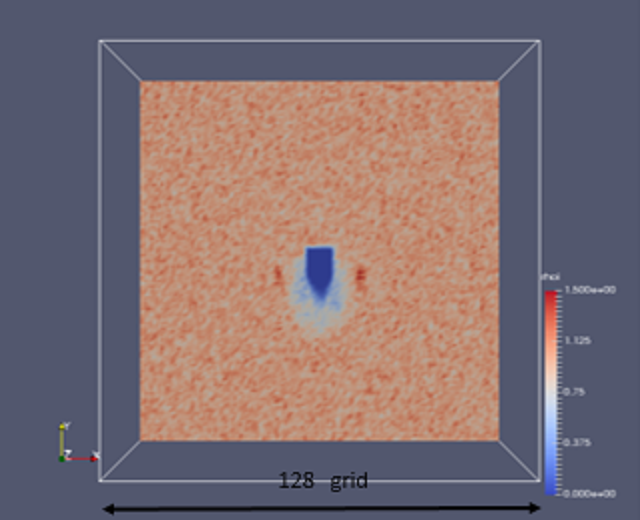
\includegraphics[width = 0.5\textwidth]{images/case3}
	        \caption{Ion density of spacecraft and surroundings without P-E. The figure on the top-left displays case 1. The top-right figure displays case 2 and the bottom-left figure displays case 3. Each
			grid point is \(1\)cm.}
			\label{fig:wake}
	    \end{figure}


\subsection{Potential difference with P-E and no P-E}
\label{sec:pot_diff}

\subsubsection{Case 1 vs case 4}

\begin{figure}
    \centering
    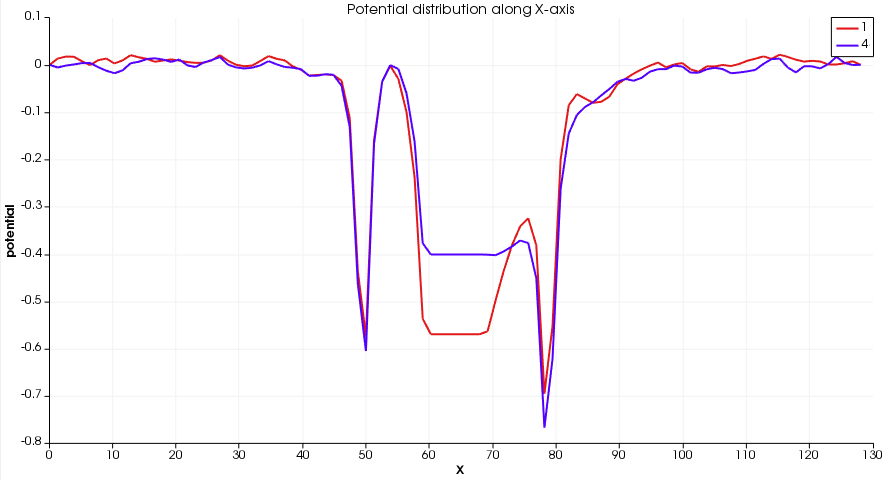
\includegraphics[width = 0.6 \textwidth]{images/pot_case14.png}
    \caption{Potential [V] of satellite and surroundings in the x-direction for case 1 and case 4. Note that the potential drop is much greater in the right probe when comparing the two cases.}
    \label{fig:pot_case14}
\end{figure}


In case 4 we have the emitted electrons in the negative flow direction. As expected this
leads to a drop in potential in the left probe which is facing the plasma flow as can be seen in figure \ref{fig:pot_case14}. The
potential drop over the probe is 0.02V or 3.8\%. The right probe is now the wake where we have
a drop in the ion density. This yields a large drop in potential compared to the left
probe, but it also has a larger potential drop than the left probe when comparing case 1 and 4. This
might be because the increase in electron density on the left side redirects more ions from the right side.
The potential drop in the right probe comparing the two cases is 0.07V or 10\%. The potential rise over the satellite is 0.17V or 28\%.


\subsubsection{Case 2 vs case 5}
\begin{figure}
    \centering
    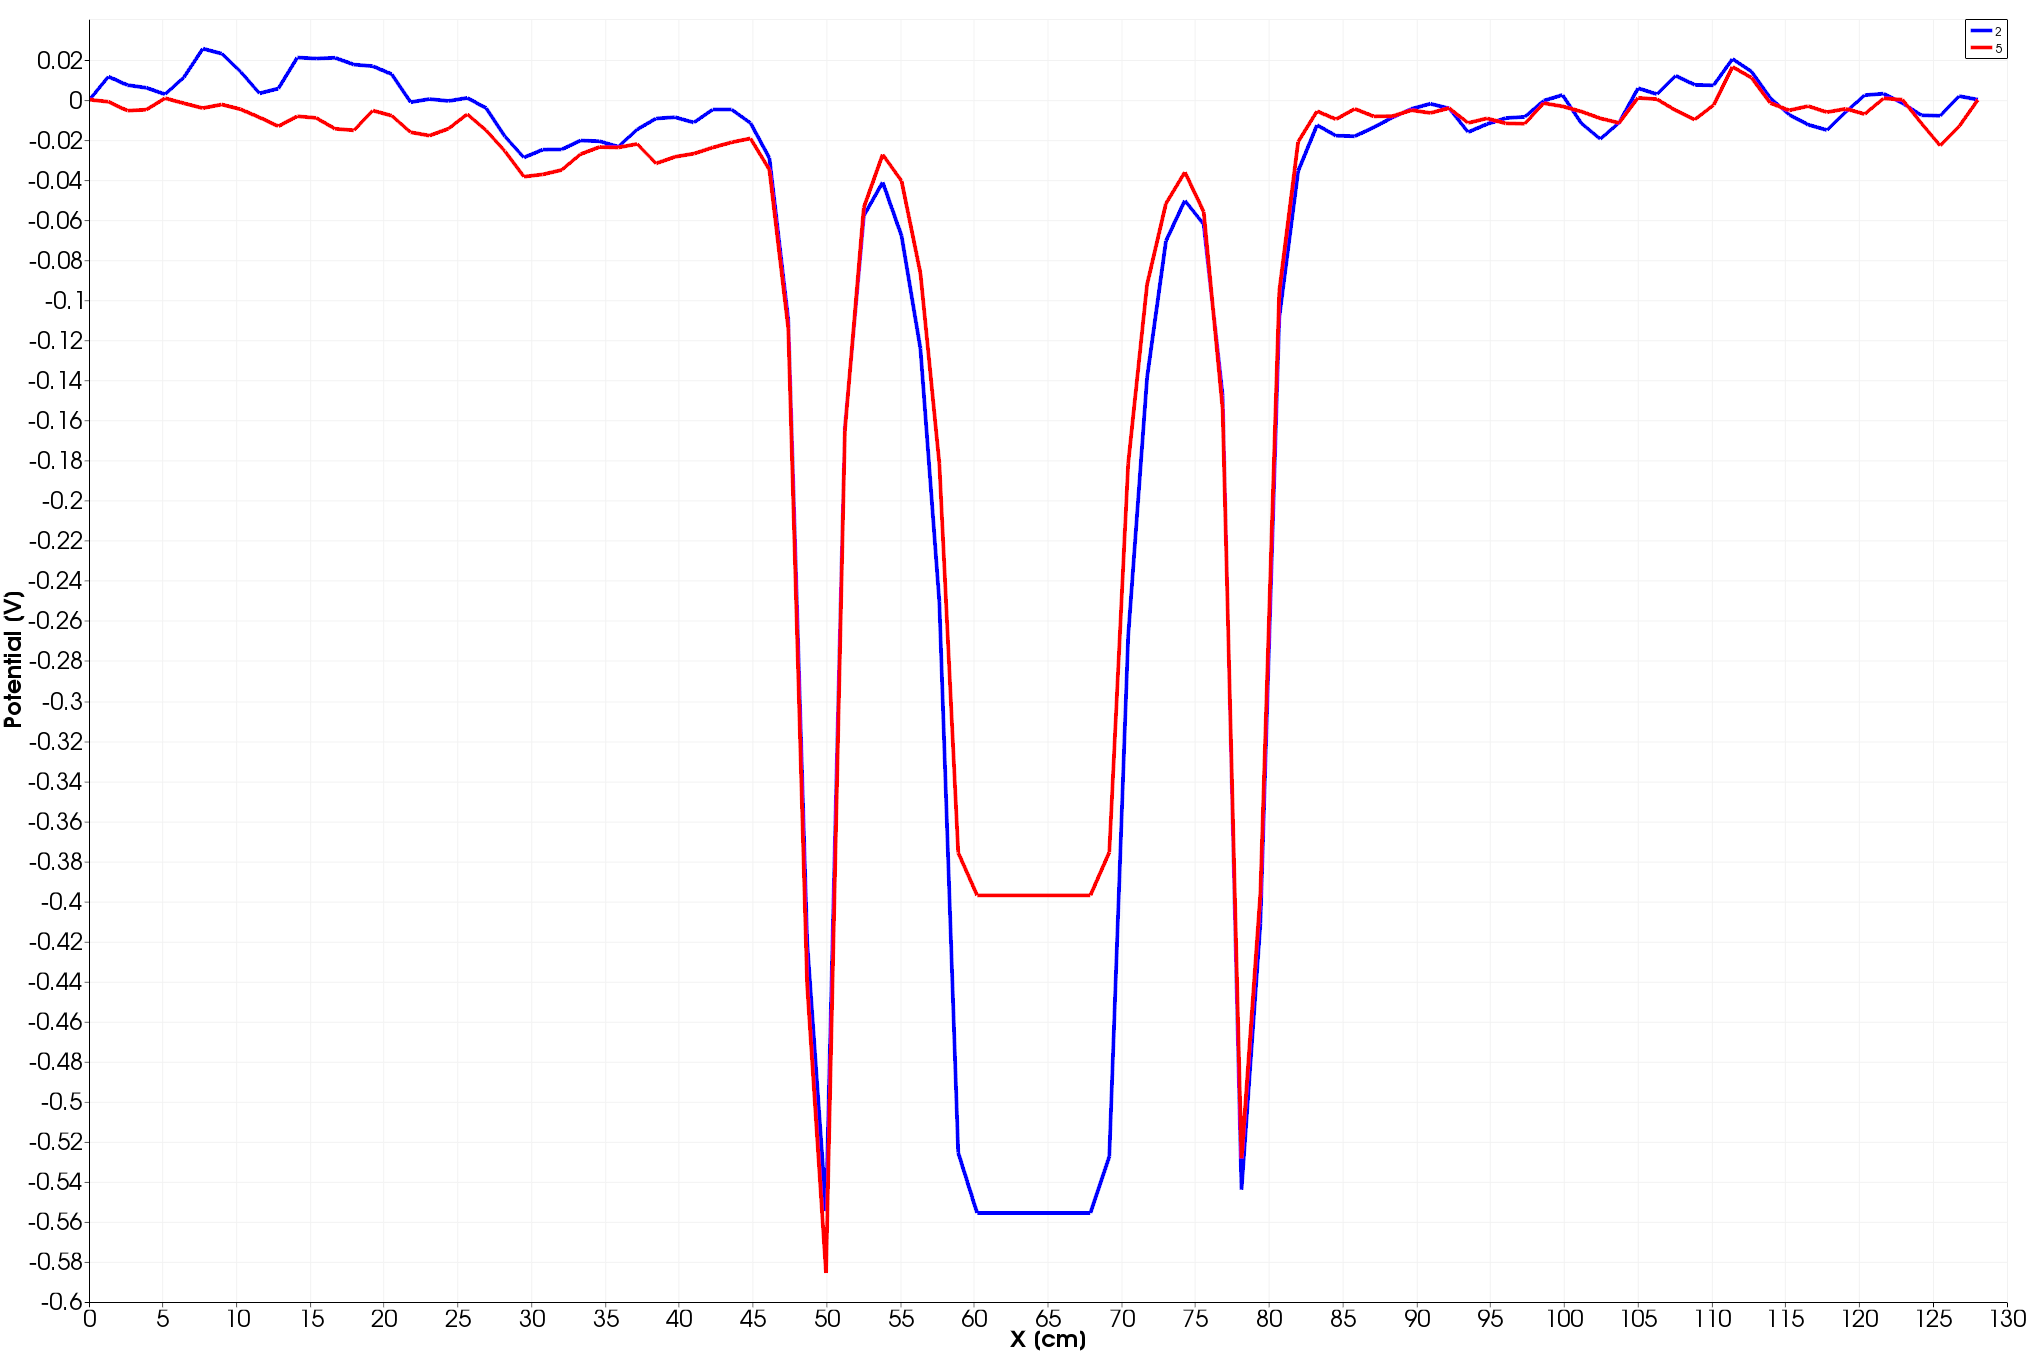
\includegraphics[width = 0.6 \textwidth]{images/pot_case25_new2.png}
    \caption{Potential of satellite and surroundings in the x-direction for case 2 and 5. Note that we have a small potential drop in the left probe but a potential rise in the right probe when comparing the two cases.}
    \label{fig:pot_case25}
\end{figure}

With the flow of emitted electrons in the negative x direction we would expect a rise in electron density around the left probe.
This can be seen in figure \ref{fig:pot_case25} where we see a 0.03V drop in the potential of this probe compared to case 5 with no emitted
electrons. On the right probe we have a small rise in the potential of 0.02V. With no emitted electrons on this side of the satellite the rise in
potential can be explained by looking at the increase in ion density as seen in figure \ref{fig:wake}.
In the satellite we have a potential rise of 0.16V which is a 28\% increase. So the change in potential in the probes are small compared to the change in the satellite.

\subsubsection{Case 3 vs case 6}

\begin{figure}
    \centering
    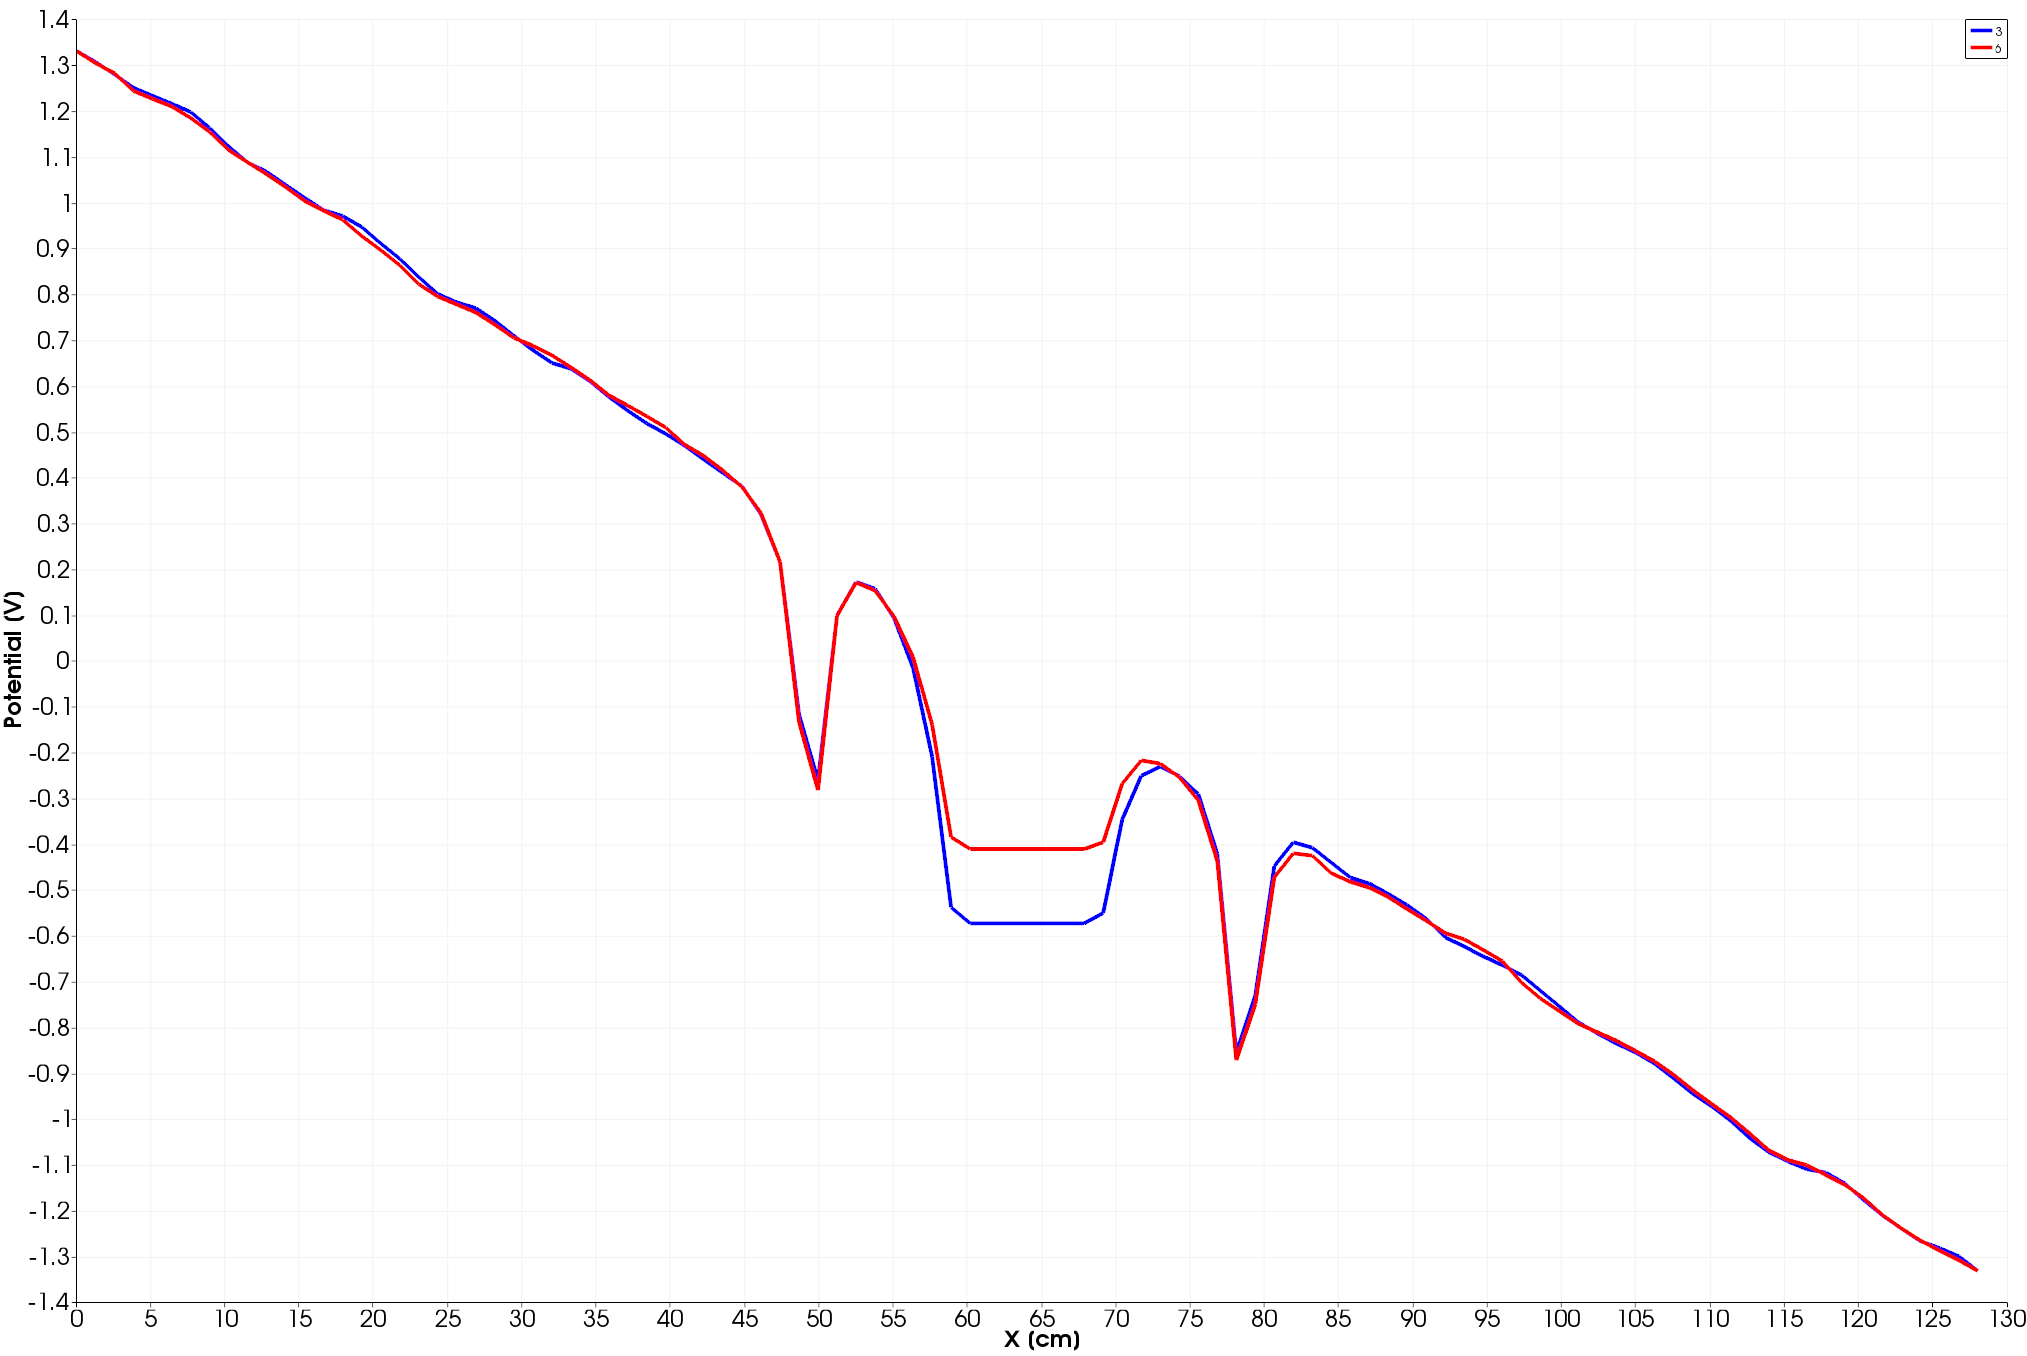
\includegraphics[width = 0.6 \textwidth]{images/pot_case36_new2.png}
    \caption{Potential of satellite and surroundings in the x-direction for case 3 and 6. Note that there is almost the same drop in potential for both probes.}
    \label{fig:pot_case36}
\end{figure}

As we can see in figure \ref{fig:pot_case36} we have almost the same change in potential over
both probes of about 0.03V. However this change yields a 12\% decrease in potential for the left
probe but a mere 3\% increase for the right probe. Over the satellite we have a potential rise of 0.15V which yields a 26\% change.
